\documentclass{beamer}
\usepackage[utf8]{inputenc}
\usepackage{amssymb}
\usepackage{amsthm}
\usepackage{amsmath}
\usepackage[utf8]{inputenc}
\usepackage{subcaption}
\usepackage{tikz}

\usetheme{Madrid}
\usecolortheme{default}

\newcommand{\uu}[0]{\mathbf{u}}
\newcommand{\kk}[0]{\mathbf{k}}
\newcommand{\ez}[0]{\mathbf{e_z}}
\newcommand{\bnabla}[0]{\boldsymbol{\nabla}}
\newcommand{\bOmega}[0]{\boldsymbol{\Omega}}
\newcommand{\pd}[2]{\frac{\partial #1}{\partial #2}}
\newcommand{\pdd}[2]{\frac{\partial^2 #1}{\partial #2^2}}


%------------------------------------------------------------
%This block of code defines the information to appear in the
%Title page
\title[Reasearch Training III] %optional
{Numerical study of stratified turbulence }

\subtitle{}

\author[Guillermin] % (optional)
{Student: Rémy~Guillermin \\ Supervisor: Pierre~Augier}

\institute[UGA] % (optional)
{
	\centering
	
\includegraphics[height=2cm]{UGA-logo.png}
}

\date[Feb 6 2025] % (optional)
{February 6, 2025}

\logo{
\includegraphics[height=1cm]{LEGI-logo}}

%End of title page configuration block
%------------------------------------------------------------



%------------------------------------------------------------
%The next block of commands puts the table of contents at the 
%beginning of each section and highlights the current section:

%\AtBeginSection[]
%{
%  \begin{frame}
%    \frametitle{Table of Contents}
%    \tableofcontents[currentsection]
%  \end{frame}
%}
%------------------------------------------------------------


\begin{document}

%The next statement creates the title page.
\frame{\titlepage}


%---------------------------------------------------------
%This block of code is for the table of contents after
%the title page
%\begin{frame}
%\frametitle{Table of Contents}
%\tableofcontents
%\end{frame}
%---------------------------------------------------------


%---------------------------------------------------------
\begin{frame}
\frametitle{Turbulence in the Atmosphere and the Ocean}

\begin{columns}
\column{0.6\textwidth}

\begin{figure}
	\centering
	\includegraphics[height=0.7\textheight]{fig/cyclone}
	\caption{Cyclone interacting over the East Pacific.}
\end{figure}

\column{0.4\textwidth}


Turbulence appears for high Reynolds number and is impacted by density stratification, temperature, salinity, etc.

\vspace{1cm}

\end{columns}
	
\end{frame}
%---------------------------------------------------------


%---------------------------------------------------------
\begin{frame}
\frametitle{Turbulence and Kolmogorov scale $\eta$}

\begin{columns}
\column{0.6\textwidth}

\begin{figure}
	\centering
	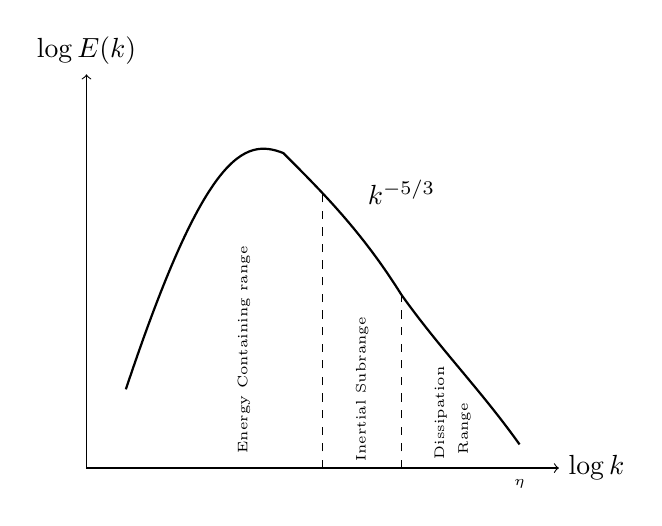
\begin{tikzpicture}
    % Axes
    \draw[->] (0,0) -- (6,0) node[right] {$\log k$};
    \draw[->] (0,0) -- (0,5) node[above] {$\log E(k)$};

    % Spectre d'énergie
    \draw[thick] (0.5,1) 
        .. controls (1.5,4) and (2,4.2) .. (2.5,4)
        .. controls (3,3.5) and (3.5,3) .. (4,2.2)
        .. controls (4.5,1.5) and (5,1) .. (5.5,0.3); 

    \draw[dashed] (3,0) -- (3,3.5);
    \draw[dashed] (4,0) -- (4,2.2);
    
    \node at (4,3.5) {$k^{-5/3}$};
    \node at (5.5,-0.2) {\tiny $\eta$};

    \node[rotate=90] at (2,1.5) {\tiny Energy Containing range};
    \node[rotate=90] at (3.5,1) {\tiny Inertial Subrange};
    \node[rotate=90] at (4.5,0.7) {\tiny Dissipation};
    \node[rotate=90] at (4.8,0.5) {\tiny Range};
	\end{tikzpicture}
\end{figure}

\column{0.4\textwidth}

\textbf{Inertital subrange:} Range where dissipation don't play a major role.

\textbf{Kolmogorov length scale $\boldsymbol{\eta}$:} Length where dissipation occurs


\vspace{1cm}

\end{columns}

	
\end{frame}
%---------------------------------------------------------


%---------------------------------------------------------
\begin{frame}
\frametitle{Density stratification}

\begin{columns}
\column{0.6\textwidth}

\begin{itemize}
	\item Forbids high vertical velocity
	\item Creates \textit{Gravity waves}
	\item Deviates from Kolmogorov $k^{-5/3}$ theory into $E(k) \propto k^{-3}$
\end{itemize}

\quad

\textbf{Brunt-Väisälä frequency $\mathbf{N}$:} $N^2 = \frac{-g}{\rho} \pd{\rho}{z}$


\column{0.4\textwidth}
\begin{figure}
	\centering
	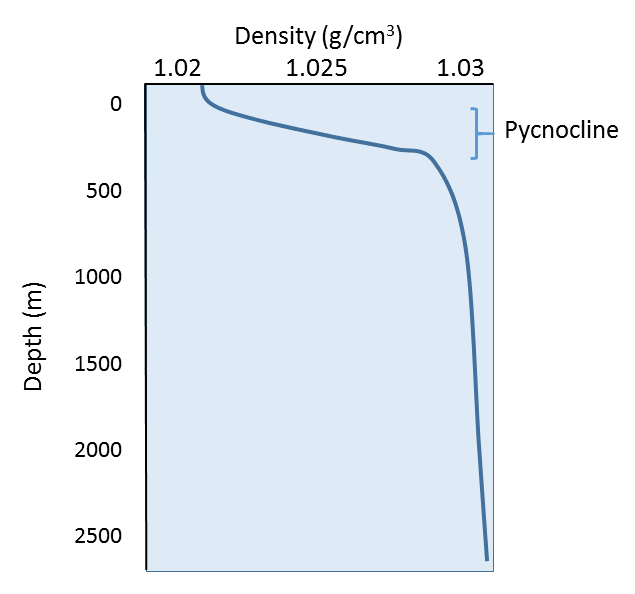
\includegraphics[width=\textwidth]{fig/density_profile.png}
	\caption{Representative density profile for the open ocean - from \textit{https://rwu.pressbooks.pub}}
\end{figure}

\vspace{1cm}

\end{columns}
	
\end{frame}
%---------------------------------------------------------


%---------------------------------------------------------
\begin{frame}
\frametitle{Navier-Stokes Equations under Boussinesq's Approximation}

\begin{align*}
	\pd{\uu}{t} + \left( \uu \cdot \bnabla \right) \uu & = - \bnabla p + b \ez + \nu \Delta \uu \\
	\bnabla \cdot \uu & = 0 \\
	\pd{b}{t} + \left( \uu \cdot \bnabla \right) b & = - N^2 u_z + \nu \Delta b
\end{align*}

\quad

\begin{itemize}
\item \textbf{Wave propagation equation:} $\partial_t^2 \uu + N^2 \Delta^{-1} \Delta_h  \uu = 0$
\item \textbf{Dispersion relation:} $\omega^2 = N^2 \sin^2{\theta}$ with $\theta = \angle(\ez, \kk)$
\end{itemize}
\end{frame}
%---------------------------------------------------------


%---------------------------------------------------------
\begin{frame}
\frametitle{Numerical Method: Framework}

\textbf{Fluidsim:} Object oriented library containing pseudo spectral solvers in \texttt{Python}

\textbf{Pseudo Spectral Method:} Equations mostly solved in Fourier space except for the non linear term.

\begin{equation*}
	\left( \uu \cdot \bnabla \right) \uu
\end{equation*}

\end{frame}
%---------------------------------------------------------



%---------------------------------------------------------
\begin{frame}
\frametitle{Numerical Method: Forcing and Simulation}

\begin{itemize}
	\item Dimension of $(3.0^2 \times 0.75)$
	\item $dx = dy = dz$
	\item Constant and localised forcing $P_k$ in the spectral space
	\item Random and isotropic initial field
	\item Condition on the viscosity: $k_{max} \eta = C$ where $C \sim 1$
\end{itemize}

\vspace{0.5 cm}

\begin{columns}
\column{0.5\textwidth}
\textbf{Maximum wavevector $\mathbf{k_{max}}$}
\column{0.5\textwidth}
\textbf{Kolmogorov length scale $\boldsymbol{\eta}$}
\end{columns}
\begin{align*}
	k_{max} = \frac{2 \pi}{L_x} \frac{n_x}{2} && \eta = \nu^{3/4} P_k^{-1/4}
\end{align*}



\end{frame}
%---------------------------------------------------------


%---------------------------------------------------------
\begin{frame}
\frametitle{Dimensionless numbers}

Characteristic turbulent velocity scale $U = (P_k L)^{1/3}$

\begin{itemize}
\item \textbf{Reynolds number:} $Re = \frac{UL_x}{\nu} = \frac{P_k^{1/3} L_x^{4/3}}{\nu}$ 
\item \textbf{Horizontal Froude number} $F_h = \frac{U}{NL_x} = \frac{P_k^{1/3}}{N L_x^{2/3}}$
\end{itemize}

\quad

High Reynolds $\implies$ More turbulence

Low Froude $\implies$ Strong stratification

\end{frame}
%---------------------------------------------------------


%---------------------------------------------------------
\begin{frame}
\frametitle{Clusters and Environment}

\textbf{Clusters available:}
\begin{itemize}
	\item \textbf{Zen (Mesonet):}  128 cores  per node
	\item \textbf{Dahu (Gricad):} 16/24/32 cores per node
\end{itemize}

\textbf{Numerical environment used:}
\begin{itemize}
	\item \texttt{Miniforge}: Easier
	\item \texttt{Guix}: Difficult to setup but mandatory for multi nodes on Dahu
\end{itemize}

\end{frame}
%---------------------------------------------------------


%---------------------------------------------------------
\begin{frame}
\frametitle{Effects of viscosity}

\begin{figure}
    \centering
    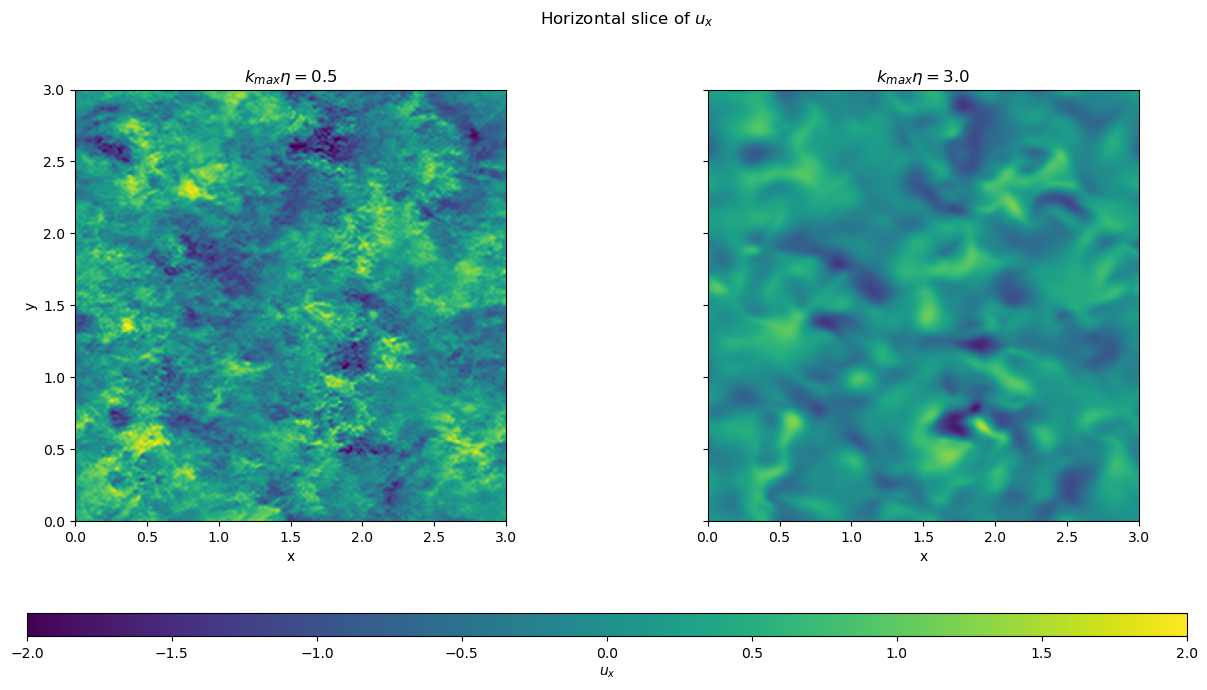
\includegraphics[height=0.65\textheight]{fig/hori_slice.png}
\end{figure}

\end{frame}
%---------------------------------------------------------


%---------------------------------------------------------
\begin{frame}
\frametitle{Effects of viscosity}

\begin{figure}
	\centering
	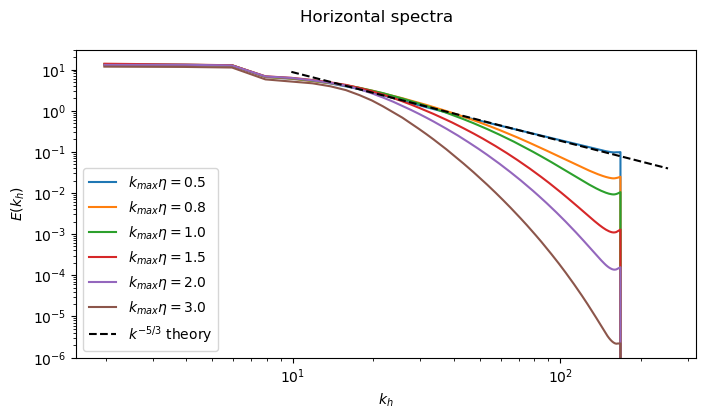
\includegraphics[height=0.7\textheight]{fig/kmax_eta.png}
\end{figure}


\end{frame}
%---------------------------------------------------------


%---------------------------------------------------------
\begin{frame}
\frametitle{Simulation results}

\begin{figure}
    \centering
    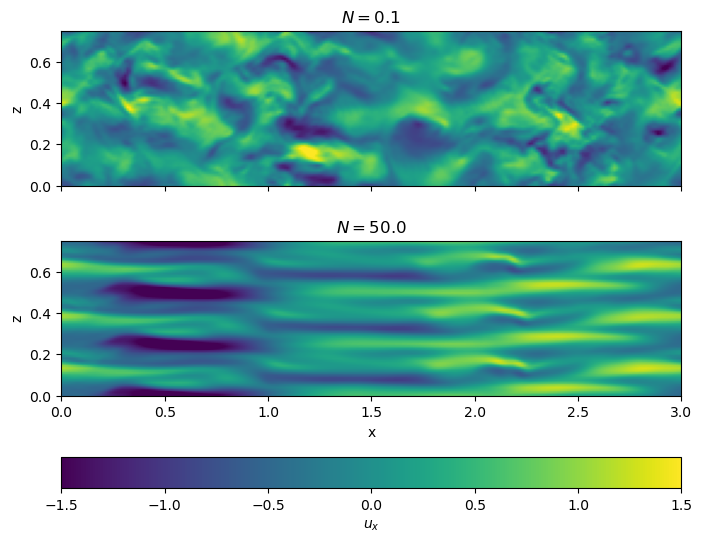
\includegraphics[height=0.65\textheight]{fig/vert_slice.png}
\end{figure}

\end{frame}
%---------------------------------------------------------


%---------------------------------------------------------
\begin{frame}
\frametitle{Simulations results}

\begin{figure}
	\centering
	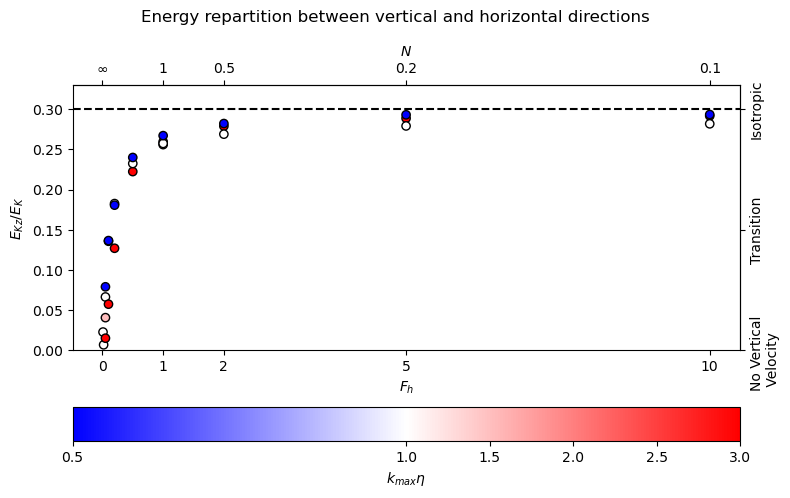
\includegraphics[width=0.85\textwidth]{fig/kz_kh.png}
\end{figure}

\end{frame}
%---------------------------------------------------------


%---------------------------------------------------------
\begin{frame}
\frametitle{Simulations results}

\begin{figure}
	\centering
	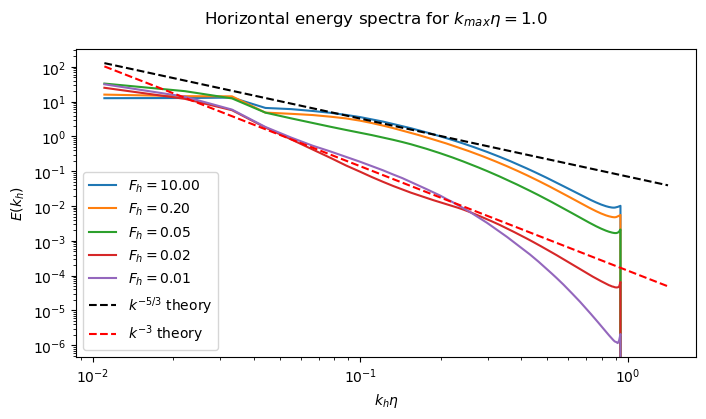
\includegraphics[width=0.85\textwidth]{fig/multi_Ekh_kh.png}
\end{figure}

\end{frame}
%---------------------------------------------------------


%---------------------------------------------------------
\begin{frame}
\frametitle{Simulations results}

\begin{figure}
	\centering
	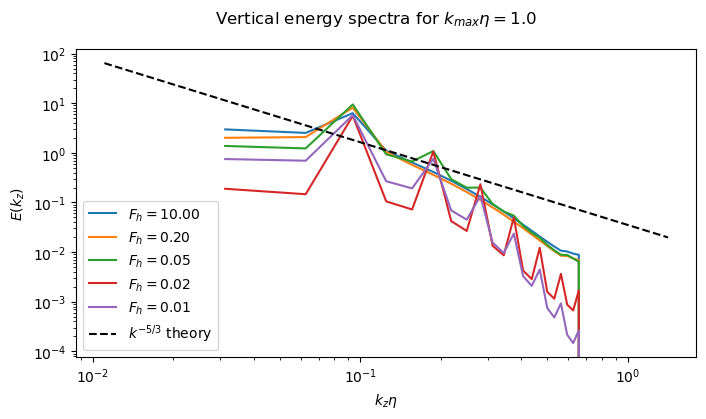
\includegraphics[width=0.85\textwidth]{fig/multi_Ekz_kz.png}
\end{figure}

\end{frame}
%---------------------------------------------------------


%---------------------------------------------------------
\begin{frame}
\frametitle{Conclusion and Discussion}

\textbf{Conclusion:}
\begin{itemize}
	\item Stratification 
	\begin{itemize}
		\item Forbids large vertical velocity
		\item Organizes the flow in layer of opposite velocity
	\end{itemize}
	\item $k_{max} \eta = 1$ is optimal
\end{itemize}

\textbf{What's next ?}
\begin{itemize}
	\item Successfully submit multi nodes job on Dahu using \texttt{Guix}
	\item Target resolution: $(1024^2 \times 256)$
\end{itemize}


\end{frame}
%---------------------------------------------------------


%---------------------------------------------------------
\begin{frame}
\frametitle{Corrupted files}

\begin{figure}
	\centering
	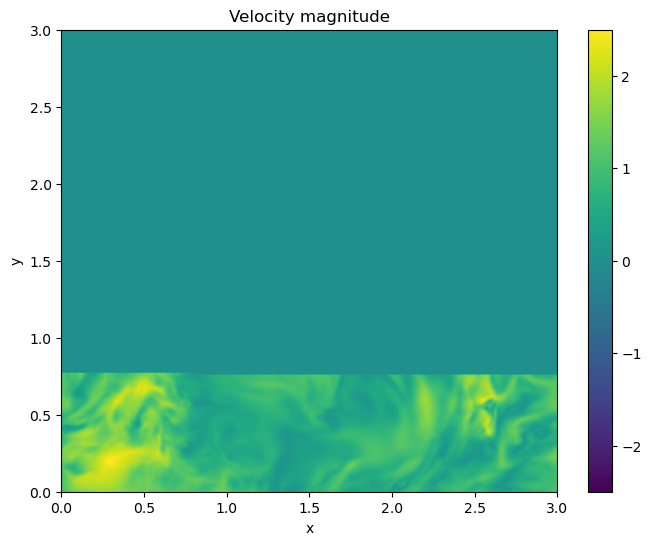
\includegraphics[width=0.8\textwidth]{fig/corrupt_slice.png}
	\caption{}
\end{figure}

\end{frame}
%---------------------------------------------------------

\end{document}